\begin{enumerate}[label=\thechapter.\arabic*,ref=\thechapter.\theenumi]
\item
For the circuit given below, choose the angular frequency $ \omega_0$ at which voltage across capacitor has maximum amplitude?
\begin{figure}[h!]
    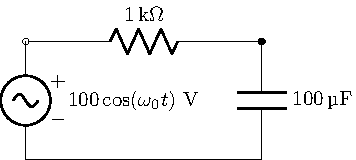
\includegraphics[width = 0.5\columnwidth]{2023/BM/16/figs/c_fig1.pdf}
    \caption{circuit }
    \centering
    \label{fig: bm_16_fig_1}
\end{figure}
\begin{enumerate}
    \item[(A)] 1000
    \item[(B)] 100
    \item[(C)] 1
    \item[(D)] 0   
\end{enumerate}
\hfill(GATE BM 2023 Question 16)\\
\item
In the following circuit, the switch S is open for $t < 0$ and closed for $t \ge 0$.
What is the steady state voltage (in Volts) across the capacitor when the switch is closed?
\begin{figure}[h!]
    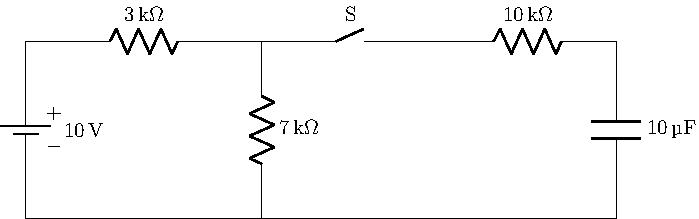
\includegraphics[width = 0.7\columnwidth]{2023/BM/30/figs/c_fig1.pdf}
    \caption{circuit }
    \centering
    \label{fig:bm_30_fig_1}
\end{figure}
\hfill(GATE BM 2023 Question 30)\\
\item 
A finite impulse response (FIR) filter has only two non-zero samples in its impulse response $h[n]$, namely $h[0] = h[1] = 1$. The Discrete Time Fourier Transform (DTFT) of $h[n]$ equals $H(e^{j\omega})$, as a function of the normalized angular frequency $\omega$. For the range $\abs{\omega} \leq \pi$, $\abs{H(e^{j\omega})}$ is equal to
\begin{enumerate}
	\item[(A)] $2\abs{\cos(\omega)}$
	\item[(B)] $2\abs{\sin(\omega)}$
	\item[(C)] $2\abs{\cos(\frac{\omega}{2})}$
	\item[(D)] $2\abs{\sin(\frac{\omega}{2})}$
\end{enumerate}
\hfill(GATE BM 2023 Question 17) \\
\item
For the circuit shown,if $i=\sin 1000t$, the instantaneous value of the Thevenin's voltage(in volts) across the terminals a anb b at time t=5ms is\\[2pt]

\begin{circuitikz}[american voltages,american currents]
    % Draw the circuit components
    \draw (0,0) -- (2,0);
    \draw (2,2) to [resistor,l=$10\Omega$] (2,4);
    \draw (2,4) -- (0,4);
    \draw (2,0) to [capacitor,l=$-j10\Omega$,-,i_=$i_x$] (2,2);
    \draw (2,0) -- (5,0);
    \draw (5,0) to[inductor,l=$j10\Omega$] (5,2);
    \draw (5,2) to [resistor,l=$10\Omega$] (5,4);
  \draw (5,4) to [cV,l^=$4i_x$,invert] (2,4);
  \draw (5,4) -- (6,4);
  \draw (6,4) to[I,l=$\sin 1000t$,invert] (6,0);
  \draw (6,0) -- (5,0);
   \node[circle,fill=black,inner sep=1.5pt,label=above:a] at (0,0) {};
    \node[circle,fill=black,inner sep=1.5pt,label=above:b] at (0,4) {};
    \end{circuitikz}
    \hfill(GATE EE 2023 Question 51) \\
\end{enumerate}
